\chapter{Experiments}

In the following chapters we discuss a series of experiments relating to the methods discussed above. 
We first discuss some experiments relating to improving the SGHMC through better estimation of the variance $\hat{V}$, and then perform some experiments related to the applicability of the methods in the context of deep learning, compared to more conventional methods.

\section{Estimating the variance}

In the SGHMC paper, they propose estimating the variance introduced through batching as $\hat{V}=0$, and then relying on the known simulated noise to make the inaccuracy of this estimate irrelevant. 
However, it seem to be worth investigating whether we could improve performance by providing some sort of estimate. 
This is also mentioned in the paper, however they do not seem explore the idea any further. 

Since we parameterized the upper bound $C$ with $\alpha$, we may end up with estimated noise larger than the upper bound. Adjusting the upper bound $C$ to accommodate this, would also require adjusting the $\alpha$ parameter accordingly. Since the $\alpha$ corresponds to the momentum decay of the algorithm, we may end up with very unstable behavior, especially for $\alpha > 1$. 
\todo[inline]{Sammenhæng mellem beta/V/B/D... skal nok rettes igennem fra teoriafdelingen.}
Instead, we keep $\alpha=CM^{-1}$ fixed, and adjust the mass matrix $M$, implictly adjusting $C$ as well.
With $M = M_0 W$ were $W$ is a diagonal matrix of weights, we can then, depending on the variance estimate, rescale the mass such that the upper bound $\alpha$ is sufficiently above the estimate $\hat\beta$, eg. by some factor $m_{\text{est}}$. If we let the learning rate be given as $\eta_0$  for the unscaled mass matrix with $W = I$, then the learning rate for the scaled system can be found as $\eta = \epsilon^2 M^{-1} = \epsilon^2 M_0^{-1}W^{-1} = \eta_0 W^{-1}$, and
\begin{align*}
    m_{\text{est}} \cdot \hat{\beta}  &\leq \alpha \Leftrightarrow\\ 
    m_{\text{est}} \cdot \frac{1}{2} \hat V \eta   &\leq \alpha \Leftrightarrow\\ 
    m_{\text{est}} \cdot \frac{1}{2} \hat V \eta_0 W^{-1}  &\leq \alpha \Leftrightarrow\\ 
    m_{\text{est}} \cdot \frac{1}{2\alpha} \hat V \eta_0   &\leq W \impliedby \\
    W_{i,i} &= \begin{cases}
        1 & \frac{1}{2\alpha}m_{\text{est}} \eta_0 \hat{V}_{i,i} < 1 \\
        \frac{1}{2\alpha}m_{\text{est}} \eta_0 \hat{V}_{i,i} & \text{otherwise}
    \end{cases}
\end{align*}

The sampler then every once in a while, eg. every 50 samples, rescales the system based on the variance estimates. If the variance estimates $\hat \beta$ happen to be greater than $\alpha$ in between the mass rescaling, the estimate is simply clamped at the upper bound $\alpha$, and no additional noise is generated.  

This method of rescaling the mass matrix is in a sense similar to the approach outlined in \cite{wenzel_how_2020}, where they also include a step calculating a preconditioning matrix, ie. $M$. They found that using the preconditioning step generally improved performance.

There are multiple ways to go about obtaining a variance estimate. We could try to calculate a running variance statistic using the within batch sample variance of the gradients:
\begin{equation}
    \frac{1}{|\tilde{\D}|-1}\sum_{(x_i,y_i)=\tilde{\D}} (\nabla U(\theta; x_i, y_i) - \nabla \bar{U}(\theta))^2
\end{equation}
and then scale the variance up to the fit the batch size. 
The main issue with this approach is that calculating the gradient for each observation individually within a batch is not really computationally sound. While it may be possible to calculate the statistic above using autograd without doing a backward pass for each observation, it is trivial to do so since autograd only allows for calculating gradients of scalars. 

Instead we look at three other approaches. 
The first approach is to run through a few training batches at the start of each epoch, calculating the gradient for each batch keeping the parameters constant. 
This estimate can then be used for the remaining epoch. 
The two other approaches instead keeps track of running statistics. 
The first uses exponentially decaying running estimates of the first to moments, $m_t, v_t$ as in the ADAM algorithm \cite{kingma_adam_2017}. Since the ADAM algorithm doesnt center the second moment estimate, the squared mean is subtracted, so that the variance is estimated as $v_t - m_t^2$.
Finally, we also try to estimate the variance as with the ADAM algorithm, however using the first momement to center the second momement estimate. 

In order to test these three different approach, they are applying to the simulated example from the previous section. Every 10 sample, the variance of the gradient is estimated using 100 random batched from the training data set. This estimate is then compared to the estimate. The estimation provided by the estimators compared to the observed variance can be seen in \cref{fig:est_variances_simulated}.
\begin{figure}[htbp]
    \centering
    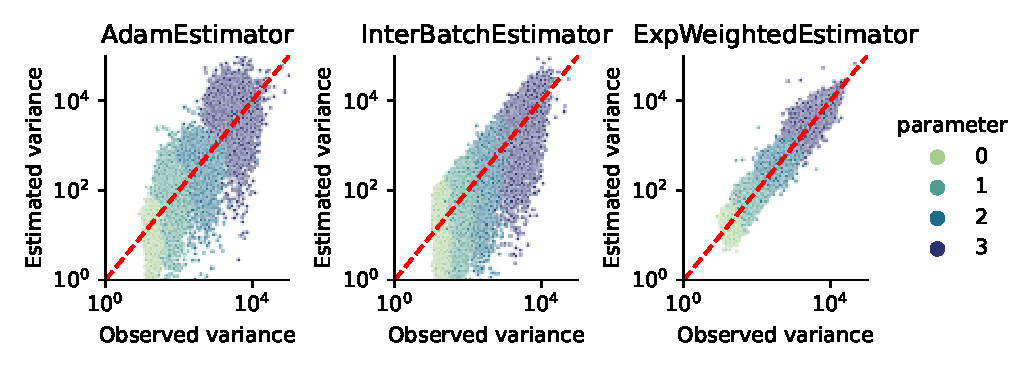
\includegraphics[width=0.9\textwidth]{Figures/simulated_sghmc_gradient_variance_estimations.pdf}
    \caption{Estimated variance compared to observed variances}
    \label{fig:est_variances_simulated}
\end{figure}
\begin{table}[htbp]
    \centering
    \begin{tabular}{lrrrr}
\toprule
parameter &    0 &    1 &    2 &    3 \\
variance\_estimator   &      &      &      &      \\
\midrule
AdamEstimator        & 0.65 & 2.03 & 1.67 & 2.98 \\
ConstantEstimator    & 1.00 & 1.00 & 1.00 & 1.00 \\
ExpWeightedEstimator & 0.30 & 0.41 & 0.42 & 0.49 \\
InterBatchEstimator  & 1.00 & 0.98 & 0.98 & 0.94 \\
\bottomrule
\end{tabular}

    \caption{Relative errors for the different estimation schemes,}
\end{table}
Note that these values are plot using a logarithmic scale, so the estimates may seem better than they actually are, especially with when it comes to overestimating. 
It may still be that they are better than simply setting $\hat\beta=0$ in terms of estimating the posterior correctly. In \cref{fig:simualted_var_est_joint_comp}, the sampled marginal distribution of $a_1$ and $a_3$ are shown again, now compared SGHMC with and without a variance estimator.
\begin{figure}[htbp]
    \centering
    \begin{subfigure}[t]{0.4\textwidth}
        \centering
        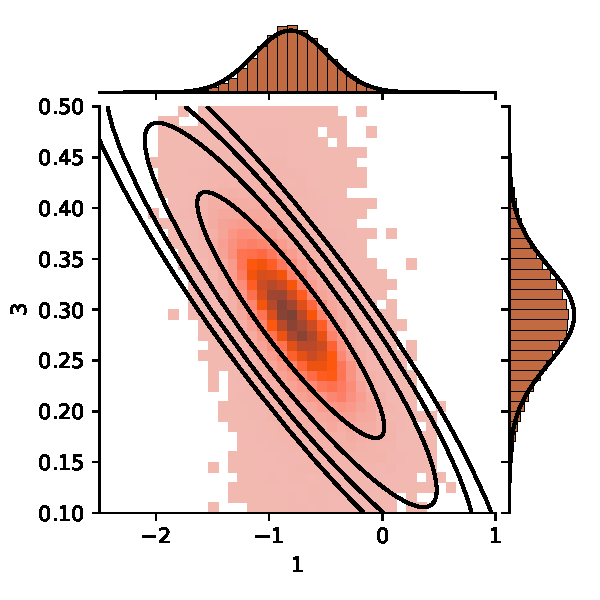
\includegraphics[width=\textwidth]{Figures/simulated_joint_SGHMC_5.pdf} 
        \caption{SGHMC with with gradient variance estimated as $\hat{V}=0$.}
    \end{subfigure}
    \begin{subfigure}[t]{0.4\textwidth}
        \centering
        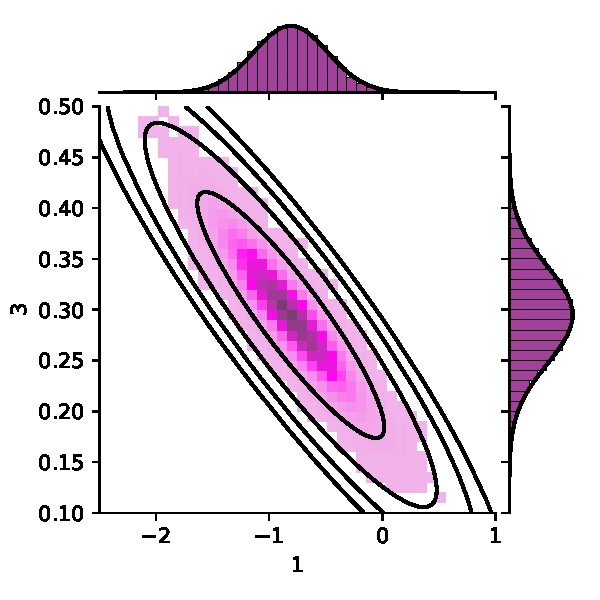
\includegraphics[width=\textwidth]{Figures/simulated_joint_SGHMCWithVarianceEstimator_5.pdf} 
        \caption{SGHMC with using the exponentially scaled estimator of gradient variance}
    \end{subfigure}
    \caption{Joint distribution of samples for $a_1$ and $a_3$ for the polynomial regression example for HMC and SGHMC for different batch sizes, with the actual posterior density also shown.}
    \label{fig:simualted_var_est_joint_comp}
\end{figure}
In this case, it does indeed seem like estimating the variance is helping the sampler.
This may come down to the approach with estimated variance is able to adjust the step size down, lowering discretization and batch error compared to SGHMC without an estimator. 

\subsection{Marginal distribution of momemtum}

In \cite{wenzel_how_2020}, they propose using the marginal distribution of the momentum as a test of the sampling assumptions. 
Per the dynamical system, if the system is simulated exactly, the marginal distribution of $r$ should be $\mathcal{N}(0, M)$. 
We should therefore have that $r M^{-1/2} \sim \mathcal{N}(0, 1)$. 
Applying the inner product, $r^T M r$ should therefore follow a $\chi^2(d)$ distribution, where $d$ is the length of $r$. 
If we look at some $c$ quantile of the $\chi^2(d)$ distribution, we would expect a fraction $c$ of the samples for $r^T M r$ to land within that particular quantile. 
To this end, let $\hat T_{0.99}$ be the fraction of samples for some set of $d$ parameters, that fall within a $0.99$ quantile of the $\chi^2(d)$ distribution. 
We should therefore expect $\hat T_{0.99}=0.99$ given a perfectly simulated system.
This allows us to test the correctness of our sampler, even if we don't know the true posterior, which is going to be the case in the following experiments.

Applying this statistic, we can see whether the estimation of the variance helps with regard to the correctness of the simulation. 
Returning back to our simulated polynomial example, in the previous experiment, the momentum were resampled every $10$ epochs, to make to comparison to regular HMC as clear as possible. 
However, if we resample the momentum from the marginal distribution too often, the $\hat{T}_{0.99}$ measure would obviously be less informative with regard to the influence of discretization and batching error. 
The momentum is therefore instead resampled every $1000$ steps, with a slighty lower learning rate of $\eta=4 \cdot 10^{-5}$.
The lower learning rate is used since otherwise, the SGHMC sampler with $\hat{\beta}=0$ becomes unstable. 
\begin{figure}[htb]
    \centering
    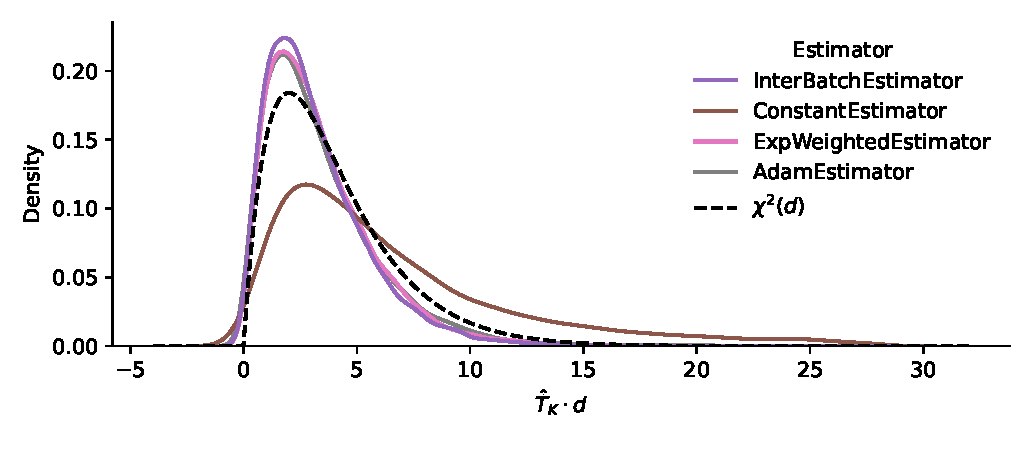
\includegraphics[width=0.9\textwidth]{Figures/temperature_sum_chi2_comp.pdf}
    \caption{<caption>}
    \label{fig:temperature_sum_chi2_comp}
\end{figure}
\begin{table}[htb]
    \centering
    \begin{tabular}{lrr}
\toprule
{} &    frac\_in\_99 &        pm \\
parameter & \multicolumn{2}{l}{linear.weight} \\
variance\_estimator   &               &           \\
\midrule
AdamEstimator        &      0.992099 &  0.001363 \\
ConstantEstimator    &      0.835864 &  0.005704 \\
ExpWeightedEstimator &      0.996358 &  0.000928 \\
InterBatchEstimator  &      0.995617 &  0.001017 \\
\bottomrule
\end{tabular}

    \caption{<caption>}
    \label{tbl:temp_99}
\end{table}
The resulting distribution of $r^T M r$ can be seen in \cref{fig:temperature_sum_chi2_comp}, compared against the expected $\chi^2$ distribution. 
We see that the while the samplers with estimated variance doesn't fit the distributional assumptions, they are all much closer than the for the sampler with $\hat \beta = 0$. The $\hat T_{0.99}$ statistic have also been calculated in \cref{tbl:temp_99}, alongside a confidence interval based on the binomial distribution.

\todo[inline]{prøv med mindre stepsize eller kom videre? Mest for at vise om varians estimation kunne afhælpe fx dårlig lr eller beta estimat. (hvilket det kunne, til dels?)}

It seem like the samplers with estimated variance are all underdispersing slighty, compared to the actual postieror. with  which would make sense if we are overestimating variance. Looking at the PLOT, the estimation margin estimates also seems relatively uniformly distributed on the log scale, which would mean that we are generally overestimating with larger magnitude. 
Since we are overestimating the noise from batching, this would lead to us not adding sufficient noise to the system, leading to underdispersion.

\section{MNIST}


\section{Convolutional Neural Net}

\subsection{CIFAR10}

\subsection{Densenet}


